\documentclass[12pt]{article}
\usepackage{amsmath}
\usepackage[english]{babel}
\usepackage{blindtext}
\usepackage{caption}
\usepackage{float}
\usepackage{graphicx}
\usepackage[utf8]{inputenc}
\usepackage{subcaption}

\title{Homework 3: Practicing with \LaTeX\ }
\author{Michelle Myers}
\date{\today}

\begin{document}

\maketitle

\section{Working with Bullets}

\subsection{Plain Bullets}
A list of things of what I enjoyed about class this semester.
\begin{itemize}
  \item The homework and tutorials were conducive to learning the
    language
  \item While maintaining their utility, the work assigned didn't
    intrude on my workload for other courses
  \item Lab sessions were good places for demonstrations 
\end{itemize}

\subsection{Numbering}
A list of what I disliked about class this semester in order of
rancor, with 1 being the worst.
\begin{enumerate}
  \item A lot of the content delivery was silly to the extent that it
    was too easy to stop taking the meetings seriously
  \item The online textbook was not maintained and updated throughout
    the progression of the course as was announced by the syllabus
  \item The random inclusion of gitHub partway through was
    off-putting. I feel like we spent way too much time going through it
\end{enumerate}

\section{Working with Equations}

\subsection{The Euler-Lagrange Equation}
This is the Euler-Lagrange equation:

\[
\sum_{j=0}^n (-1)^j \partial_{ \mu_{1}\ldots\mu_{j} }^j\left(\frac{
    \partial \mathcal{L} }{\partial f_{i, \mu_1 \dots \mu_{j} } }\right
  ) = 0 
\]
where $\mu_{1}\ldots \mu_{j}$ implies the sum over indices that span the
number of variables.

\section{Working with Tables}

\begin{table}[h!]
  \centering
  \begin{tabular}{ c | c | c }
    \hline
    Favorite Foods & Favorite Bands & Favorite IDL Commands \\ \hline
    Rib-Eye Steaks & Muse & oplot \\
    Vinaigrette Salads & Abd al Malik & return \\
    Spinach & Elton John & print \\ \hline
  \end{tabular}
  \caption{ Steak and Salad are the bomb, with Spinach somewhere in the mix in honor of the great legend Popeye. }
\end{table}

\section{Working with a Figure}
I will demonstrate to you an image. Prepare to be amazed...
\begin{figure}[H]
  \centering
  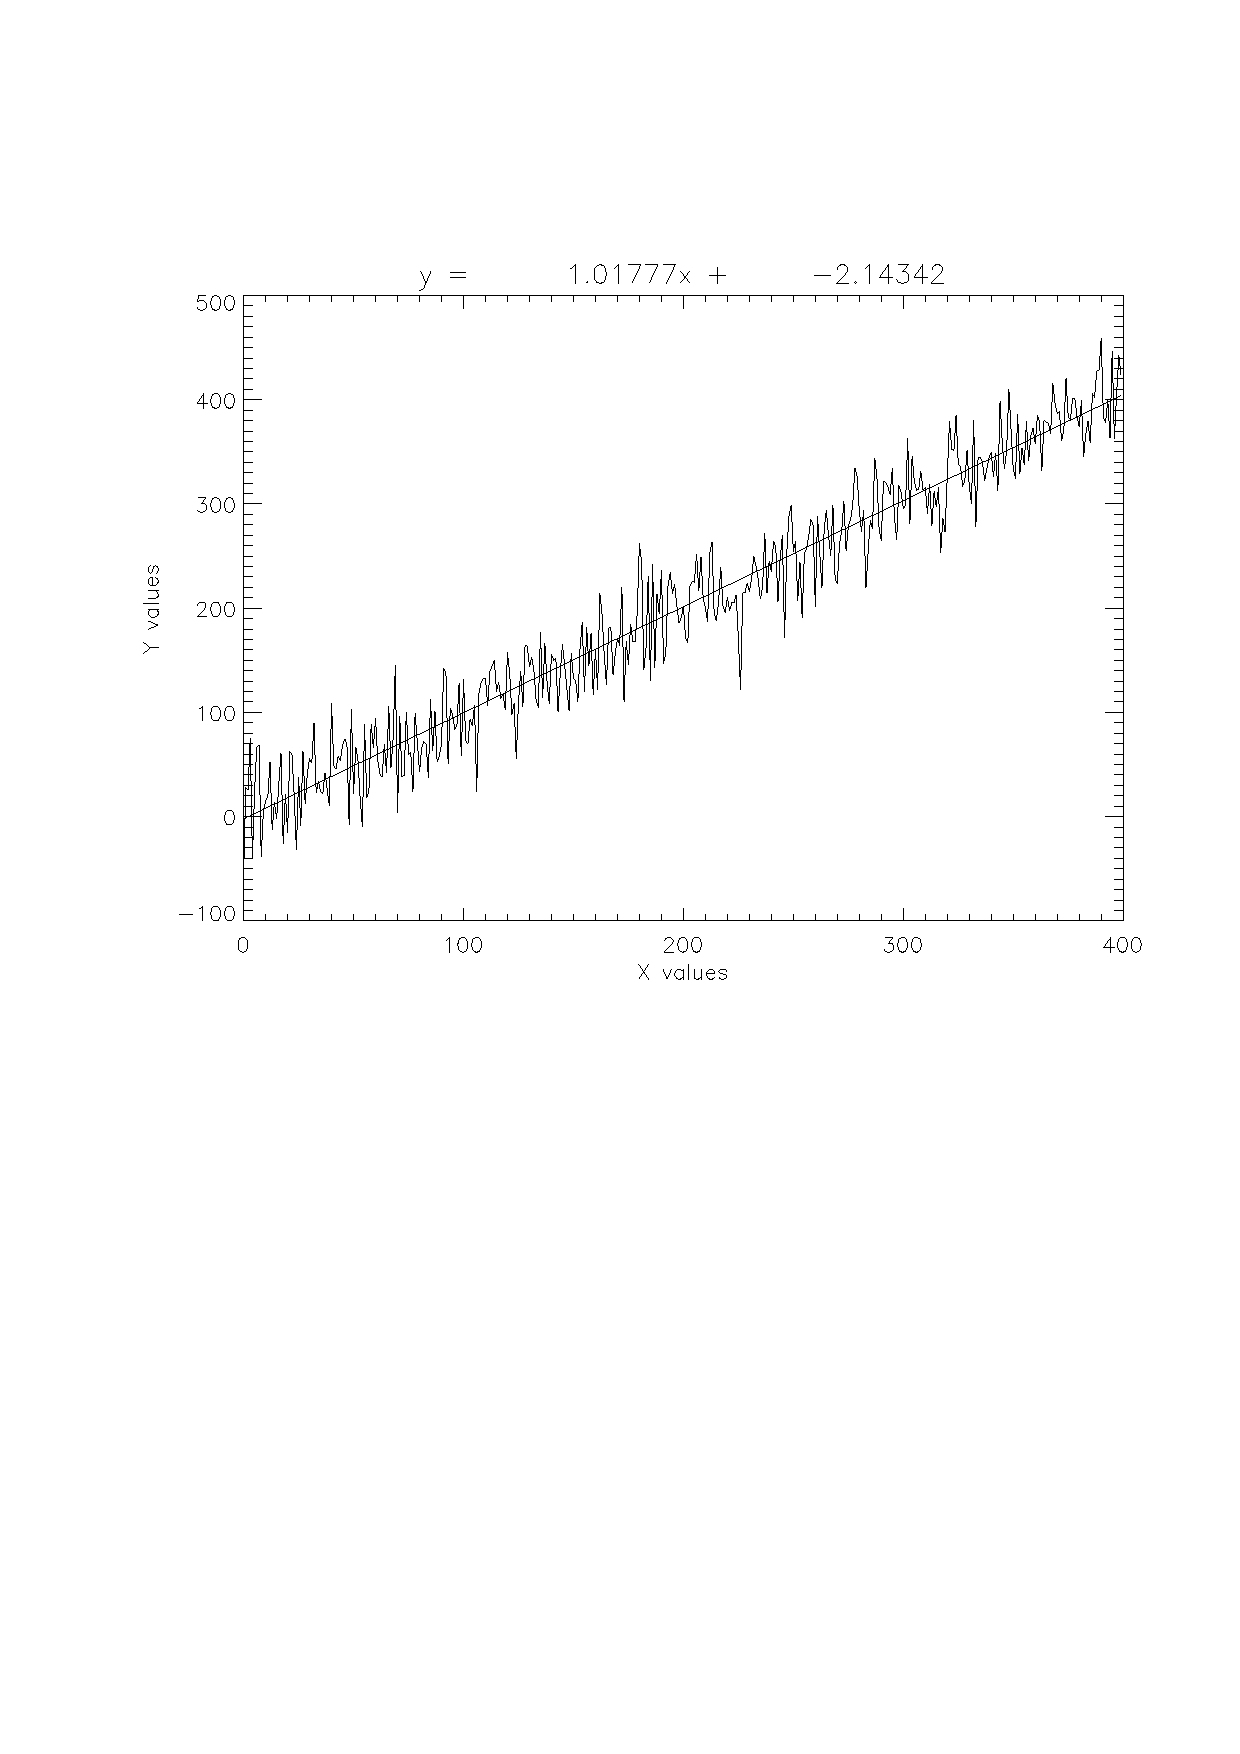
\includegraphics[width=0.5\textwidth]{tut6.pdf}
  \caption{A linear fit of a data file. Be amazed.}
\end{figure}

\section{Working with Multiple Figures}
I'm hungry, 'nuff said.
\begin{figure}[H]
  \centering

  \begin{subfigure}[h!]{0.4\textwidth}
    \includegraphics[width=\textwidth]{ribeye.jpg}
    \caption{One half of a well-balanced meal}
  \end{subfigure}
  ~
  \begin{subfigure}[h!]{0.4\textwidth}
    \includegraphics[width=\textwidth]{salad.jpg}
    \caption{The other half of a well-balanced meal}
  \end{subfigure}
  \caption{The best things in life}

\end{figure}
\end{document}
